\documentclass[tikz]{standalone}
\usepackage{tikz}
\usetikzlibrary{positioning, graphs, matrix}
\usetikzlibrary{graphs.standard}
\begin{document}
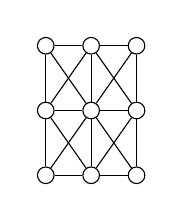
\begin{tikzpicture}
		[mynode/.style={draw, circle, inner sep = 0mm, minimum size = 0.6em}]
		\matrix[row sep = 1.7em, column sep = 1em]{
			\node[mynode] (1) {}; & \node[mynode] (2) {}; & \node[mynode] (3) {}; \\
			\node[mynode] (8) {}; & \node[mynode] (9) {}; & \node[mynode] (4) {}; \\
			\node[mynode] (7) {}; & \node[mynode] (6) {}; & \node[mynode] (5) {}; \\
		};
		\foreach \i [evaluate={\j=int(mod(\i, 8) + 1)}] in {1, 2, ..., 8}{
			\draw (\i) -- (\j);
			\draw (\i) -- (9);
		}
		\foreach \i [evaluate={\j=int(mod(\i, 8) + 2)}] in {2, 4, 6, 8}{
			\draw (\i) -- (\j);
		}
\end{tikzpicture}
\end{document}